\documentclass[10pt,review,sigplan,anonymous=true,authorversion=true,nonacm=true]{acmart}
\settopmatter{printfolios=false,printccs=false,printacmref=false}

\bibliographystyle{ACM-Reference-Format}
\citestyle{acmauthoryear}   %% For author/year citations
\usepackage{listings,multirow,wrapfig,xspace,paralist}
\usepackage{xcolor,tikz,graphicx, pifont}
%\usetikzlibrary{positioning}

%% \newcommand{\authorcomment}[3]{\xspace\textcolor{#1}{{\bf #2} #3}\xspace}
\newcommand{\authorcomment}[3]{}
% For author notes:
\newcommand{\AG}[1]{\authorcomment{orange}{AG}{#1}}
\newcommand{\JV}[1]{\authorcomment{red}{JV}{#1}}

% For meta comments:
\newcommand{\isit}[1]{\authorcomment{cyan}{Check}{#1}}
\newcommand{\todo}[1]{\authorcomment{red}{TODO}{#1}}
\newcommand{\xmark}{\textcolor{red}{\ding{55}}}
\newcommand{\cmark}{\textcolor{green}{\ding{51}}}

\definecolor{LightGray}{RGB}{247, 247, 247}
\definecolor{Gray}{rgb}{.3,.3,.3}
\definecolor{DarkGray}{rgb}{.5,.5,.5}

%% https://www.davehofmann.de/defining-custom-language-templates-for-latex-listings/
% Define Language
\lstdefinelanguage{smalleR} {
  % list of keywords
  morekeywords={
    for,
    if,
    else,
    function
  },
  sensitive=true, % keywords are not case-sensitive
  morecomment=[l]{\#}, % l is for line comment
  morestring=[b]{"} % defines that strings are enclosed in double quotes
}

\lstset{
  language={smalleR},
  columns=flexible,
  captionpos=b,
  frame=single,
  framerule=0pt,
  framexleftmargin=1mm,
  framexrightmargin=1mm,
  tabsize=2,
  belowskip=0pt,
  basicstyle=\small\ttfamily,
  backgroundcolor=\color{LightGray},
  emphstyle=\sffamily,
  keywordstyle=\bfseries,
  commentstyle=\color{Gray}\em,
  stringstyle=\color{Gray},
  alsoletter={., _, $},
  breaklines=true
}

\newcommand{\code}[1]{\lstinline |#1|\xspace}
\renewcommand{\c}[1]{\lstinline |#1|\xspace}
\newcommand{\eg}{\emph{e.g.},\xspace}
\newcommand{\ie}{\emph{i.e.},\xspace}

\newcommand{\environmentFun}{\code{environment}}
\newcommand{\asEnvironment}{\code{as.environment}}

\newcommand{\emptyenv}{\code{empyenv}}
\newcommand{\globalenv}{\code{globalenv}}

\newcommand{\base}{\code{base}}
\newcommand{\methods}{\code{methods}}
\newcommand{\lazyLoadDBexec}{\code{lazyLoadDBexec}}

\newcommand{\newEnv}{\code{new.env}}

\newcommand{\asList}{\code{as.list}}
\newcommand{\listToEnv}{\code{list2env}}

\newcommand{\ls}{\code{ls}}
\newcommand{\objects}{\code{objects}}

\newcommand{\subDollar}{\code{$}}
\newcommand{\subBracket}{\code{[[}}

\newcommand{\exist}{\code{exist}}

\newcommand{\get}{\code{get}}
\newcommand{\getZero}{\code{get0}}
\newcommand{\mget}{\code{mget}}
\newcommand{\dynGet}{\code{dynGet}}

\newcommand{\assign}{\code{assign}}

\newcommand{\remove}{\code{remove}}
\renewcommand{\rm}{\code{rm}}

\newcommand{\lockEnvironment}{\code{lockEnvironment}}
\newcommand{\lockBinding}{\code{lockBinding}}
\newcommand{\unlockBinding}{\code{unlockBinding}}

\newcommand{\eval}{\code{eval}}
\newcommand{\substitute}{\code{substitute}}

\newcommand{\parentEnv}{\code{parent.env}}
\newcommand{\parentEnvAssign}{\code{parent.env<-}}

\newcommand{\envtracer}{{\sf envtracer}\xspace}
\newcommand{\experimentr}{{\sf experimentr}\xspace}
\newcommand{\rdyntrace}{{\sf R-dyntrace}\xspace}

\newcommand{\ggplot}{\textit{ggplot2}\xspace}
\newcommand{\vctrs}{\textit{vctrs}\xspace}

%%% \setcopyright{rightsretained}
%%% \acmPrice{}
%%% \acmDOI{10.1145/3360579}
%%% \acmYear{2019}
%%% \copyrightyear{2019}
%%% \acmJournal{PACMPL}
%%% \acmVolume{3}
%%% \acmNumber{OOPSLA}
%% \acmArticle{153}
%%% \acmMonth{10}
\begin{document}
\title{On Design and Use of First-Class Environments in R}

\author{Aviral Goel}\affiliation{\institution{Northeastern University}\country{USA}}
\author{Jan Vitek}\affiliation{\institution{Czech Technical University and Northeastern University}\country{USA}}
\authorsaddresses{}
\renewcommand{\shortauthors}{Goel, et al.}


\begin{abstract}
  The R programming language is widely used for statistical computing. To enable
  interactive data exploration and rapid prototyping, R encourages a dynamic
  programming style. This programming style is support by a number of features
  including first-class environments. R is the only language, with millions of
  users, that provides a full reflective interface for manipulating
  environments. With the great flexibility afforded by first-class environments,
  comes challenges for reasoning about code and significant restrictions about
  what transformations a compiler is allowed to apply to programs. This paper is
  an overview of the environment interface refined over two decades. We explain
  the rationale behind the design and document how environments are used in the
  wild by the means of a corpus analysis.
\end{abstract}

\begin{CCSXML}
<ccs2012>
<concept>
<concept_id>10002944.10011123.10010912</concept_id>
<concept_desc>General and reference~Empirical studies</concept_desc>
<concept_significance>500</concept_significance>
</concept>
<concept>
<concept_id>10011007.10011006.10011008</concept_id>
<concept_desc>Software and its engineering~General programming languages</concept_desc>
<concept_significance>500</concept_significance>
</concept>
<concept>
<concept_id>10011007.10011006.10011050.10010517</concept_id>
<concept_desc>Software and its engineering~Scripting languages</concept_desc>
<concept_significance>500</concept_significance>
</concept>
<concept>
<concept_id>10011007.10011006.10011039.10011311</concept_id>
<concept_desc>Software and its engineering~Semantics</concept_desc>
<concept_significance>300</concept_significance>
</concept>
</ccs2012>
\end{CCSXML}

\ccsdesc[500]{General and reference~Empirical studies}
\ccsdesc[500]{Software and its engineering~General programming languages}
\ccsdesc[500]{Software and its engineering~Scripting languages}
\ccsdesc[300]{Software and its engineering~Semantics}

%\keywords{R language, delayed or lazy evaluation}

\maketitle
\section{Introduction}

The ability to name values in a computation is a key building block of
linguistic abstractions. Programming languages have concepts such as local
variables, global variables, function parameters that boil down to a mapping
of values to names, commonly referred to as an \emph{environment}. The semantics of
environments have a profound impact on how programming languages can be
implemented. At a first approximation, restricted semantics greatly simplify the
task of generating efficient machine code.

Early languages had variables that were read and written to by statically
determined names, and they did not support recursive functions. Thus there was a
single environment for compilation unit and, in that environment, each variable
its own memory location; as it generated code the compiler knew exactly which
location every name referred to. When a variable's value was constant, that
variable could be treated as a synonym for its value and did not require a
memory location. To improve performance, variables could be cached in machine
registered and spilled to memory only when needed.

As languages became more expressive, allowing recursion and first-class
functions, implementations had to allocate environments, respectively, on the
stack or in the heap. Lisp treated code as data, and thus lifted the restriction
that variable names be statically known. This meant that from a compiler's point
of view, it became much harder to generate efficient code. Environments were
data structures that could at any time be inspected and the mapping between
variables and values be observed.

In this paper, we focus on the R programming language created in 1993~\cite{r96}, as
a directed descendent to S whose origin dates to 1976~\cite{s88}. Inspired by Lisp,
CLOS, and Scheme, the designers of R created a lazy functional language that
supported various forms of object-oriented programming. One of the keys to
expressivity was the choice of making environments first-class. Environments are
data structures that can be created and manipulated programmatically. One can,
for example, write code that acquires the environment of the caller of the
currently executing function, check if it contains a variable named \c{x}, and,
if it does, rename that variable to \c{y}. Needless to say that this flexibility
does limit what a compiler can do to make R run fast~\cite{dls19}.

Our goal with this paper is to document the interface that R exposes to
environments. This interface evolved through the years, some of it dates back to
S, with changes and adaptations through the decades. The interface is rich and
not always consistent or certainly not minimal. Through a dynamic analysis
conducted on a corpus of popular R libraries and their clients, we report on the
practical usage of environments. This allows us to explain the need for this
rich interface and could, possibly, be a step towards a re-design or a hint for
compiler writers as to where optimization opportunities may lie.

\section{Related Work}

While the Scheme Standard specifies that the \code{eval} function takes an
environment-specifier, this need not be a first-class
environment~\cite{SchemeR5RS}. The effect of assignment to variables in this
environment is unspecified, leaving open the possibility of it being immutable.
GNU Scheme supports first-class environments and, as a consequence, its
\code{eval} takes an explicit environment. It provides functions to create new
environments, read and write bindings, examine parent environments, and obtain
the current environment as a reified value. Python provides the \code{locals}
function that returns the local bindings as a dictionary, attached to the
current frame as an attribute. Updates to this dictionary are not reflected in
the function's scope. Caller's bindings can be accessed from their frame
obtained by calling \code{inspect.stack}. Calling \code{locals} outside of a
function returns the namespace as a dictionary at the point and changes to this
dictionary are reflected in the namespace. Python's \code{globals} returns a
dictionary of the global namespace whose updates are also reflected in the
namespace.

\citet{NishizakiSTLC94} introduced a simply typed lambda calculus with
first-class environments, proved that it is strongly normalizing, and proposed a
type inference algorithm. \citet{NishizakiML94} proposed a sound type inference
algorithm for a type system with ML-polymorphism in a $\lambda$-calculus with
first-class environments.

\citet{ecoop12} discussed the design of R, providing a comprehensive explanation
of R's scoping and evaluation mechanism. They present many aspects of
environments in the context of laziness, metaprogramming, dynamic evaluation,
explicit environment manipulation, and call stack inspection, but they don't
discuss explicit environment creation using \code{new.env}. In comparison to
their work, our work focuses only on environments and provides a much more
detailed qualitative and quantitative account. Furthermore, our study shows a
significantly larger and richer use of explicit environments in the R ecosystem
compared to theirs. \citet{oopsla19b} studied the design and use of laziness in
R. They provide a detailed account of the language’s evaluation strategy with a
small-step operational semantics and an empirical evaluation of laziness in
16,707 packages. Their semantics shows that promises are stored in environments
and can outlive the frame that created them if returned as part of that
environment. \citet{oopsla20b} inferred type signatures for R functions by
observing the type of argument and return values. Their type language includes a
type for first-class environments.


\section{Environments in the R Language}

The evolution of R has been gradual, rather than offering clearly delineated
abstractions, the language designer opened up the internals of the interpreter
for all to see, and packaged some commonly needed functionality into functions
bundled with the core of the language. Thus, the task of describing the
``interface'' of environments as seen by developers and end-users involves quite
a lot of sleuthing. As we prepared this paper, we kept discovering new functions
that accessed environments from native code. This section is not meant to be an
exhaustive description, but it gives an overview of the most commonly used
functions that manipulate environments.

%R is a dynamic language with first-class, lexically scoped, functions.
\subsection{The R language}

A presentation of the language requires introducing some key concepts. We will
be brief, interested readers should consult~\cite{AdvancedR}.

\paragraph{Functions} Functions are first-class, anonymous, lexically-scoped values
with optional parameters and default values. R is ``functional'' in the sense
that values have a copy-on-write semantics, so that side-effects to arguments
inside a function are not reflected to the caller.

\paragraph{Promises} R is a mostly lazy language.  Arguments to functions are
packaged into promises which bundle an expression and its environment. When the
value of a promise is needed, the expression is evaluated in the adjoined
environment and the result is cached in the promise.

\paragraph{Vectors}  Most values in R are vectors, and most operations are
vectorized. Vectors are homogeneous arrays of integer, double,
character, logical, complex, or raw values.

\paragraph{Lists} Lists are heterogeneous vectors with optionally named elements.
They can be indexed by position or name. Lists (and vectors) have a
copy-on-write semantics, but the language maintains a reference count and allows
mutation in place when a value is not aliased.


\paragraph{Attributes}
Values can be tagged with user-defined attributes which are a map from string to
value. Consider the following code which sets the attributes \code{dim} and
\c{class} of some vector \code{x}.

\begin{lstlisting}
  x <- c(1,2,3,4)
  attr(x, dim) <- c(2,2)
  class(x) <- c("cat")
\end{lstlisting}

Setting the \code{dim} attribute causes the vector to be subsequently treated as
a 2$\times$2 matrix. Similarly, the class attribute is used for method dispatch
in an object-oriented style.

\paragraph{Formulas}  A formula is a compact symbolic
representation of models used by statistical functions. For example, the linear
model \code{y~x-1} specifies a line through the origin. Each formula contains a
reference to the environment in which it is defined to refer to the variables,
if they are not otherwise provided during model fitting.

\paragraph{Environments}
Environments bind names to values, implemented by an association list or a
hashmap, chosen at construction. Each environment also has a parent, forming an
acyclic chain terminated by the empty environment. That environment is returned
by \code{emptyenv()}. Unlike other values, environments are mutable.

\subsection{Environments as Packages}

Packages loaded by calls to \code{library()} are represented as environments;
their names are added to a global search path (returned by \code{search()}). The
\emph{n}-th package environment can be retrieved using \code{pos.to.env(n)}, or
\code{as.environment(n)}. \asEnvironment also accepts the package name as its
argument. Every package has a corresponding namespace environment which also
contains its private bindings and implementation specific metadata. The
namespace environment for a package \code{P} can be obtained by calling
\code{getNamespace(P)}. An R session starts with the base package preloaded,
which contains the default R APIs. \code{baseenv()} returns the base package
environment and binds \code{.BaseNamespaceEnv} to that environment.

\subsection{Environments as Scopes}
The top-level scope is the \code{global} environment, referred by the variable
\code{.GlobalEnv}, or returned by \code{globalenv()}. The \code{environment()}
call returns the current evaluation environment which is either the
\code{global} environment or the current function's environment. When supplied
with a function argument, it returns the function's definition environment.
\code{environment(f)<-e} sets \code{e} as the environment of \code{f}.

\begin{lstlisting}
 f <- function() print(environment())
 environment(); environment(f); f()
 # <env: Global> <env: Global> <env: 0x7ff>
 e <- new.env()
 print(e)
 # <env: 0x7f1>
 environment(f) <- e
 environment(f)
 # <env: 0x7f1>
\end{lstlisting}

\noindent
R provides a call stack reflection interface. Frame number starts from 0, for
\code{global} environment (top level), and increases by 1 for each nested call.
\code{sys.nframe()} returns the current frame number. \code{sys.parent(n)}
returns the frame number of the \code{n}th parent. The function
\code{sys.frame(n)} returns the environment of the frame at position \code{n}
(counting backwards if \code{n} is negative). Function \code{parent.frame(n)} is
an optimized implementation of \code{sys.frame(sys.parent(n))}. Lastly,
\code{sys.frames()} returns a list of all active frames' environments.

\begin{lstlisting}
 f <- function() { print(environment())
 g <- function() { parent.frame(1); g() }
 f()
 # <env: 0x7f2> <env: 0x7f2>
\end{lstlisting}

\subsection{Environments as Data Structures}

Environments can be created using the \newEnv function. This function takes
three optional arguments: a boolean to select a hash table representation over
the default association list, a size for preallocation, and, an enclosing
environment. R does not provide any function to query the representation used
for an environment. The \code{length} function returns the number of bindings in
an environment. \parentEnv yields the enclosing environment and
\code{parent.env(e)<-p} sets the enclosing environment of \code{e} to \code{p}.

\begin{lstlisting}
  e <- new.env(parent=emptyenv())
  length(e)
  # 0
  parent.env(e)
  # <environment: R_EmptyEnv>
  parent.env(e) <- globalenv()
  parent.env(e)
  # <environment: R_GlobalEnv>
\end{lstlisting}

\asList converts environments to lists; in R lists can associate names with
elements. \listToEnv copies the elements of a list to an environment. If the
environment is not supplied, it creates one using \newEnv. The variables of an
environment can be retrieved as a vector using the \ls and \objects functions.

\begin{lstlisting}
  l <- list(x=1, y=2); e <- list2env(l)
  length(e)
  # 2
  as.list(e)
  # list(y = 2, x = 1)
  ls(e)
  # [1] "x" "y"
\end{lstlisting}

\noindent
A variable's existence in an environment can be queried using \exist. Its value
can be retrieved using \subDollar and \subBracket operators. \get, \getZero,
\mget, and \dynGet functions are generalizations of these operators with options
to perform lookup recursively in parent environments (\code{inherits = TRUE})
and validate the type of value bound to the variable being read (\code{mode =
  "integer"}). \getZero is \get with an extra argument, \code{ifnotfound}, which
is returned if the variable is not present in the environment. \mget is a
vectorized version of \get; it reads multiples variables supplied as a vector
and returns a vector of values. \dynGet performs recursive lookups in caller
frames, i.e., dynamic scopes, unlike the other functions which perform lookups in
lexical scopes.

Writes can be performed in an environment using the \assign function. Operator
forms, \code{env$var <- val}, and \code{env[["var"]] <- val}, can also be used
for mutating variable \code{var} in environment \code{env}. Bindings
can be removed from an environment using the \rm and \remove function.

An environment can be protected from the addition or removal of bindings by
locking it with \lockEnvironment. This does not protect existing bindings from
modification, which can be explicitly locked using \lockBinding. A locked
binding can be removed if the environment is not locked. Bindings can be
unlocked using \unlockBinding.

Expressions can be evaluated explicitly in an environment using the \eval
function. To support metaprogramming, R provides the \substitute function. This
function extracts the unevaluated argument text from the promise bound to the
argument in the supplied environment.

\paragraph{Discussion.}
R provides a large API for interactive with environments and accessing scopes as
explicit environments. Environments in R are very versatile objects. While they
primarily serve as scopes, they can also be used as hash tables, and sandboxing
expression evaluation. Though R is lexically scoped, ad-hoc lookup strategies
can be implemented by accessing arbitrary caller environments. The lexical scope
of a function can be changed, a technique often used for designing custom
object-oriented systems.

\section{Analysis Infrastructure}

In this section, we describe the infrastructure that will be used for dynamic
analysis. This infrastructure has three main tasks: assembling executable
programs from R packages, generating execution traces using an modified R
interpreter, and post-processing the traces to generate graphs and statistics.
The entire pipeline is managed by a Makefile that invokes R scripts for each
step. Trace collection and analysis steps are parallelized using GNU
Parallel~\cite{gnuparallel}. For reproducibility, the infrastructure is
installed in a container, based on Debian 10.9, and executed on Docker.

\subsection{Assembling a Corpus}

The corpus of executable programs is assembled from R packages hosted on CRAN,
the official R package repository. Our scripts mirror CRAN on the analysis
server and install its packages. Another script invokes the R APIs that
locate and extract examples, tests, and vignettes from these packages. These
programs are then prepared for tracing by wrapping them in a call to the tracer.
Another set of scripts computes metadata such as lines of code from the
installed packages and extracted corpus.

\subsection{Generating Execution Traces}

Execution traces are generated using \envtracer, a dynamic analyzer built on top
of \rdyntrace. \rdyntrace is a modified GNU R virtual machine version
4.0.2~\cite{oopsla19b} that raises events during program execution. Callbacks
attached to these events receive relevant R objects at that point of execution.
\envtracer uses these callbacks to collect execution information associated with
environments. The events used by \envtracer include function entry and exit,
eval entry and exit, object allocation and deallocation, package loading and
attaching, variable lookup, assignment, and removal, subassignment, subsetting,
and attribute setting. On tracing entry, \envtracer initializes the tracing
state. When the program is about to exit \envtracer stores the traces in a
tabular format for post-processing. While the setup is conceptually simple, the
details are complex, and, affect scalability if not handled correctly. To handle
the subtleties of R, \envtracer maintains models of concrete R objects, such as
environments, functions, calls, and frames on the call stack. Model objects have
unique identities, whereas R objects are identified by their memory address, and
the garbage collector can reuse these. \envtracer takes care memory management
for model objects and provides efficient indexing. \envtracer heuristically
constructs names of model functions. The model stack updates itself
appropriately in response to longjump used by R for non-local returns.
Furthermore, \envtracer extends these models with custom fields which are
updated in response to \rdyntrace events for collecting data related to this
paper.

\subsection{Post-processing}
In the post-processing step, the execution traces are analyzed to gather
insights about the use of environments. \envtracer gathers 681GB of data from
the corpus. Scale is the major challenge. We use a custom map-reduce style
analysis to process this data. First, in the \textit{reduce} phase, the
individual execution traces are partially summarized in parallel to generate
smaller data tables per program, per analysis. This is the most expensive step
and it substantially reduces the data size. Second, in the \textit{combine}
phase, these tables are concatenated into a single table per analysis. Third, in
the \textit{summarize} phase, final summaries are computed from the concatenated
tables. Finally, in the \textit{report} phase, graphs and tables are generated
from these summaries using R Markdown notebooks~\cite{rmdpkg}.

\subsection{Our Corpus of R Programs}

For this study, we assembled a corpus of 100 most widely used packages from
CRAN~\cite{ligges2017}, based on the number of client packages. These packages
together have 11,786 clients. Package \ggplot has the highest number of clients,
2,320, and package \vctrs has the fewest, 108. These packages contribute 481.5K
lines of R code and 1M lines of native code. During execution, these 100
packages call functions from 186 other packages, so our evaluation also includes
them. These extra packages have 478.2K lines of R code and 1.1M lines of native
code.


\begin{table}[!h]
  \vspace{-3mm}
  \small
  \centering
  \caption{Corpus}\label{table:corpus}
  \vspace{-3mm}
  \begin{tabular}{lrrr}
    \toprule
    &\bf Tests&\bf Examples&\bf Vignettes\\
    \midrule
    {Scripts}&1.9K&5.0K&187.0\\
    \midrule
    {LOC}&136.7K&55.2K&13.9K\\
    \bottomrule
  \end{tabular}
\end{table}

CRAN packages come equipped with runnable code in the form of tests, examples,
and long-form examples called vignettes. These programs are extracted as
independently executable scripts for evaluation by the \experimentr library.
Experiments demonstrate the use of a package's functions, and vignettes
illustrate a package's functionality with a larger example, typically using data
supplied with the package. Table~\ref{table:corpus} presents the number and size
of these scripts. Overall, there are 6.9K scripts with 205.8K lines of code.

The 286 corpus packages have 44.3K top-level functions, of which, 18.7K
functions are exercised by the extracted scripts. From the un-exercised 25.6K
functions, the majority, 17.2K, belong to transitively included packages, and,
8.4K belong to the initially selected 100 packages. Since the executable scripts
are extracted from 100 packages, they don't provide good coverage for the
transitively included 186 packages.

Table~\ref{table:fundist} presents the distribution of exercised functions
across these packages. We observe that 171 packages have 25 functions or less.
There are few large packages; 8 packages have more than 500 functions.

\begin{table}[!h]
  \vspace{-2mm}
  \small
  \caption{Package Size} \label{table:packsize}
  \centering
  \begin{tabular}{lr}
    \toprule
    \bf Functions&\bf Packages\\
    \midrule
    1--25&169\\
    26--50&40\\
    51--100&17\\
    101--150&14\\
    151--200&11\\
    201--250&15\\
    \bottomrule
  \end{tabular}
  \quad
  \begin{tabular}{lr}
    \toprule
    \bf Functions&\bf Packages\\
    \midrule
    251--300&4\\
    301--400&6\\
    401--500&2\\
    501--600&3\\
    601--700&0\\
    701--800&3\\
    \bottomrule
  \end{tabular}
\end{table}

We observed 42.1M calls to these functions. Figure~\ref{fig:calldist} shows the
distribution of calls. 52.9\% functions are called more than ten times. 14.3\%
functions are called only once, leading to low coverage.

\begin{figure}[!h]
  \centering
  % Created by tikzDevice version 0.12.3.1 on 2021-06-03 17:14:17
% !TEX encoding = UTF-8 Unicode
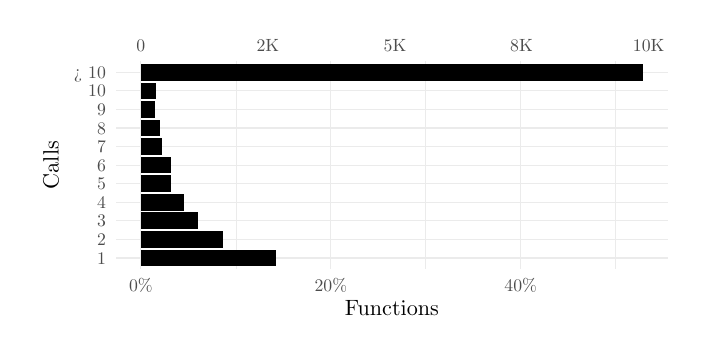
\begin{tikzpicture}[x=1pt,y=1pt]
\definecolor{fillColor}{RGB}{255,255,255}
\path[use as bounding box,fill=fillColor,fill opacity=0.00] (0,0) rectangle (238.49,108.41);
\begin{scope}
\path[clip] ( 31.86, 21.16) rectangle (231.38, 96.31);
\definecolor{drawColor}{gray}{0.92}

\path[draw=drawColor,line width= 0.2pt,line join=round] ( 75.23, 21.16) --
	( 75.23, 96.31);

\path[draw=drawColor,line width= 0.2pt,line join=round] (143.83, 21.16) --
	(143.83, 96.31);

\path[draw=drawColor,line width= 0.2pt,line join=round] (212.43, 21.16) --
	(212.43, 96.31);

\path[draw=drawColor,line width= 0.4pt,line join=round] ( 31.86, 25.19) --
	(231.38, 25.19);

\path[draw=drawColor,line width= 0.4pt,line join=round] ( 31.86, 31.90) --
	(231.38, 31.90);

\path[draw=drawColor,line width= 0.4pt,line join=round] ( 31.86, 38.61) --
	(231.38, 38.61);

\path[draw=drawColor,line width= 0.4pt,line join=round] ( 31.86, 45.32) --
	(231.38, 45.32);

\path[draw=drawColor,line width= 0.4pt,line join=round] ( 31.86, 52.03) --
	(231.38, 52.03);

\path[draw=drawColor,line width= 0.4pt,line join=round] ( 31.86, 58.73) --
	(231.38, 58.73);

\path[draw=drawColor,line width= 0.4pt,line join=round] ( 31.86, 65.44) --
	(231.38, 65.44);

\path[draw=drawColor,line width= 0.4pt,line join=round] ( 31.86, 72.15) --
	(231.38, 72.15);

\path[draw=drawColor,line width= 0.4pt,line join=round] ( 31.86, 78.86) --
	(231.38, 78.86);

\path[draw=drawColor,line width= 0.4pt,line join=round] ( 31.86, 85.57) --
	(231.38, 85.57);

\path[draw=drawColor,line width= 0.4pt,line join=round] ( 31.86, 92.28) --
	(231.38, 92.28);

\path[draw=drawColor,line width= 0.4pt,line join=round] ( 40.93, 21.16) --
	( 40.93, 96.31);

\path[draw=drawColor,line width= 0.4pt,line join=round] (109.53, 21.16) --
	(109.53, 96.31);

\path[draw=drawColor,line width= 0.4pt,line join=round] (178.13, 21.16) --
	(178.13, 96.31);
\definecolor{fillColor}{RGB}{0,0,0}

\path[fill=fillColor] ( 40.93, 89.26) rectangle (222.31, 95.30);

\path[fill=fillColor] ( 40.93, 22.17) rectangle ( 89.89, 28.21);

\path[fill=fillColor] ( 40.93, 28.88) rectangle ( 70.62, 34.92);

\path[fill=fillColor] ( 40.93, 35.59) rectangle ( 61.56, 41.63);

\path[fill=fillColor] ( 40.93, 42.30) rectangle ( 56.31, 48.34);

\path[fill=fillColor] ( 40.93, 55.72) rectangle ( 51.90, 61.75);

\path[fill=fillColor] ( 40.93, 49.01) rectangle ( 51.87, 55.04);

\path[fill=fillColor] ( 40.93, 62.43) rectangle ( 48.49, 68.46);

\path[fill=fillColor] ( 40.93, 69.13) rectangle ( 47.87, 75.17);

\path[fill=fillColor] ( 40.93, 82.55) rectangle ( 46.25, 88.59);

\path[fill=fillColor] ( 40.93, 75.84) rectangle ( 46.18, 81.88);
\end{scope}
\begin{scope}
\path[clip] (  0.00,  0.00) rectangle (238.49,108.41);
\definecolor{drawColor}{gray}{0.30}

\node[text=drawColor,anchor=base,inner sep=0pt, outer sep=0pt, scale=  0.64] at ( 40.85, 99.91) {0};

\node[text=drawColor,anchor=base,inner sep=0pt, outer sep=0pt, scale=  0.64] at ( 86.78, 99.91) {2K};

\node[text=drawColor,anchor=base,inner sep=0pt, outer sep=0pt, scale=  0.64] at (132.72, 99.91) {5K};

\node[text=drawColor,anchor=base,inner sep=0pt, outer sep=0pt, scale=  0.64] at (178.45, 99.91) {8K};

\node[text=drawColor,anchor=base,inner sep=0pt, outer sep=0pt, scale=  0.64] at (224.39, 99.91) {10K};
\end{scope}
\begin{scope}
\path[clip] (  0.00,  0.00) rectangle (238.49,108.41);
\definecolor{drawColor}{gray}{0.30}

\node[text=drawColor,anchor=base east,inner sep=0pt, outer sep=0pt, scale=  0.64] at ( 28.26, 22.98) {1};

\node[text=drawColor,anchor=base east,inner sep=0pt, outer sep=0pt, scale=  0.64] at ( 28.26, 29.69) {2};

\node[text=drawColor,anchor=base east,inner sep=0pt, outer sep=0pt, scale=  0.64] at ( 28.26, 36.40) {3};

\node[text=drawColor,anchor=base east,inner sep=0pt, outer sep=0pt, scale=  0.64] at ( 28.26, 43.11) {4};

\node[text=drawColor,anchor=base east,inner sep=0pt, outer sep=0pt, scale=  0.64] at ( 28.26, 49.82) {5};

\node[text=drawColor,anchor=base east,inner sep=0pt, outer sep=0pt, scale=  0.64] at ( 28.26, 56.53) {6};

\node[text=drawColor,anchor=base east,inner sep=0pt, outer sep=0pt, scale=  0.64] at ( 28.26, 63.24) {7};

\node[text=drawColor,anchor=base east,inner sep=0pt, outer sep=0pt, scale=  0.64] at ( 28.26, 69.95) {8};

\node[text=drawColor,anchor=base east,inner sep=0pt, outer sep=0pt, scale=  0.64] at ( 28.26, 76.66) {9};

\node[text=drawColor,anchor=base east,inner sep=0pt, outer sep=0pt, scale=  0.64] at ( 28.26, 83.37) {10};

\node[text=drawColor,anchor=base east,inner sep=0pt, outer sep=0pt, scale=  0.64] at ( 28.26, 90.08) {> 10};
\end{scope}
\begin{scope}
\path[clip] (  0.00,  0.00) rectangle (238.49,108.41);
\definecolor{drawColor}{gray}{0.30}

\node[text=drawColor,anchor=base,inner sep=0pt, outer sep=0pt, scale=  0.64] at ( 40.93, 13.15) {0{\%}};

\node[text=drawColor,anchor=base,inner sep=0pt, outer sep=0pt, scale=  0.64] at (109.53, 13.15) {20{\%}};

\node[text=drawColor,anchor=base,inner sep=0pt, outer sep=0pt, scale=  0.64] at (178.13, 13.15) {40{\%}};
\end{scope}
\begin{scope}
\path[clip] (  0.00,  0.00) rectangle (238.49,108.41);
\definecolor{drawColor}{RGB}{0,0,0}

\node[text=drawColor,anchor=base,inner sep=0pt, outer sep=0pt, scale=  0.80] at (131.62,  4.40) {Functions};
\end{scope}
\begin{scope}
\path[clip] (  0.00,  0.00) rectangle (238.49,108.41);
\definecolor{drawColor}{RGB}{0,0,0}

\node[text=drawColor,rotate= 90.00,anchor=base,inner sep=0pt, outer sep=0pt, scale=  0.80] at ( 11.20, 58.73) {Calls};
\end{scope}
\end{tikzpicture}

  \caption{Call Distribution}
  \label{fig:calldist}
\end{figure}

These functions have a total of 67,225 parameter positions.
Figure~\ref{fig:paramdist} shows the distribution of parameter positions. 3.0\%
functions have 0 parameters, 22.4\% have 1, and 5.0\% have over 10. There are 4
functions with over 50 parameters that come from 3 packages. Of those,
\texttt{ggplot2::theme} has the highest, 95 parameters.

\begin{figure}[!h]
  \centering
  % Created by tikzDevice version 0.12.3.1 on 2021-06-03 17:14:19
% !TEX encoding = UTF-8 Unicode
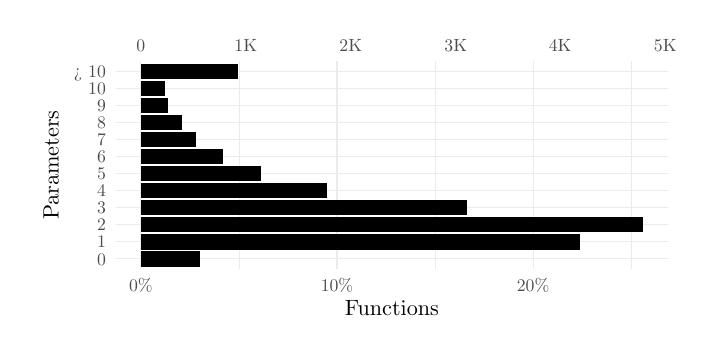
\begin{tikzpicture}[x=1pt,y=1pt]
\definecolor{fillColor}{RGB}{255,255,255}
\path[use as bounding box,fill=fillColor,fill opacity=0.00] (0,0) rectangle (238.49,108.41);
\begin{scope}
\path[clip] ( 31.86, 21.16) rectangle (231.38, 96.31);
\definecolor{drawColor}{gray}{0.92}

\path[draw=drawColor,line width= 0.2pt,line join=round] ( 76.35, 21.16) --
	( 76.35, 96.31);

\path[draw=drawColor,line width= 0.2pt,line join=round] (147.19, 21.16) --
	(147.19, 96.31);

\path[draw=drawColor,line width= 0.2pt,line join=round] (218.04, 21.16) --
	(218.04, 96.31);

\path[draw=drawColor,line width= 0.4pt,line join=round] ( 31.86, 24.86) --
	(231.38, 24.86);

\path[draw=drawColor,line width= 0.4pt,line join=round] ( 31.86, 31.02) --
	(231.38, 31.02);

\path[draw=drawColor,line width= 0.4pt,line join=round] ( 31.86, 37.18) --
	(231.38, 37.18);

\path[draw=drawColor,line width= 0.4pt,line join=round] ( 31.86, 43.34) --
	(231.38, 43.34);

\path[draw=drawColor,line width= 0.4pt,line join=round] ( 31.86, 49.50) --
	(231.38, 49.50);

\path[draw=drawColor,line width= 0.4pt,line join=round] ( 31.86, 55.66) --
	(231.38, 55.66);

\path[draw=drawColor,line width= 0.4pt,line join=round] ( 31.86, 61.81) --
	(231.38, 61.81);

\path[draw=drawColor,line width= 0.4pt,line join=round] ( 31.86, 67.97) --
	(231.38, 67.97);

\path[draw=drawColor,line width= 0.4pt,line join=round] ( 31.86, 74.13) --
	(231.38, 74.13);

\path[draw=drawColor,line width= 0.4pt,line join=round] ( 31.86, 80.29) --
	(231.38, 80.29);

\path[draw=drawColor,line width= 0.4pt,line join=round] ( 31.86, 86.45) --
	(231.38, 86.45);

\path[draw=drawColor,line width= 0.4pt,line join=round] ( 31.86, 92.61) --
	(231.38, 92.61);

\path[draw=drawColor,line width= 0.4pt,line join=round] ( 40.93, 21.16) --
	( 40.93, 96.31);

\path[draw=drawColor,line width= 0.4pt,line join=round] (111.77, 21.16) --
	(111.77, 96.31);

\path[draw=drawColor,line width= 0.4pt,line join=round] (182.62, 21.16) --
	(182.62, 96.31);
\definecolor{fillColor}{RGB}{0,0,0}

\path[fill=fillColor] ( 40.93, 89.84) rectangle ( 76.18, 95.38);

\path[fill=fillColor] ( 40.93, 22.09) rectangle ( 62.34, 27.63);

\path[fill=fillColor] ( 40.93, 28.25) rectangle (199.57, 33.79);

\path[fill=fillColor] ( 40.93, 83.68) rectangle ( 49.80, 89.22);

\path[fill=fillColor] ( 40.93, 34.41) rectangle (222.31, 39.95);

\path[fill=fillColor] ( 40.93, 40.56) rectangle (158.76, 46.11);

\path[fill=fillColor] ( 40.93, 46.72) rectangle (108.20, 52.27);

\path[fill=fillColor] ( 40.93, 52.88) rectangle ( 84.25, 58.43);

\path[fill=fillColor] ( 40.93, 59.04) rectangle ( 70.64, 64.59);

\path[fill=fillColor] ( 40.93, 65.20) rectangle ( 60.94, 70.75);

\path[fill=fillColor] ( 40.93, 71.36) rectangle ( 55.94, 76.91);

\path[fill=fillColor] ( 40.93, 77.52) rectangle ( 50.67, 83.06);
\end{scope}
\begin{scope}
\path[clip] (  0.00,  0.00) rectangle (238.49,108.41);
\definecolor{drawColor}{gray}{0.30}

\node[text=drawColor,anchor=base,inner sep=0pt, outer sep=0pt, scale=  0.64] at ( 40.85, 99.91) {0};

\node[text=drawColor,anchor=base,inner sep=0pt, outer sep=0pt, scale=  0.64] at ( 78.80, 99.91) {1K};

\node[text=drawColor,anchor=base,inner sep=0pt, outer sep=0pt, scale=  0.64] at (116.74, 99.91) {2K};

\node[text=drawColor,anchor=base,inner sep=0pt, outer sep=0pt, scale=  0.64] at (154.69, 99.91) {3K};

\node[text=drawColor,anchor=base,inner sep=0pt, outer sep=0pt, scale=  0.64] at (192.43, 99.91) {4K};

\node[text=drawColor,anchor=base,inner sep=0pt, outer sep=0pt, scale=  0.64] at (230.38, 99.91) {5K};
\end{scope}
\begin{scope}
\path[clip] (  0.00,  0.00) rectangle (238.49,108.41);
\definecolor{drawColor}{gray}{0.30}

\node[text=drawColor,anchor=base east,inner sep=0pt, outer sep=0pt, scale=  0.64] at ( 28.26, 22.65) {0};

\node[text=drawColor,anchor=base east,inner sep=0pt, outer sep=0pt, scale=  0.64] at ( 28.26, 28.81) {1};

\node[text=drawColor,anchor=base east,inner sep=0pt, outer sep=0pt, scale=  0.64] at ( 28.26, 34.97) {2};

\node[text=drawColor,anchor=base east,inner sep=0pt, outer sep=0pt, scale=  0.64] at ( 28.26, 41.13) {3};

\node[text=drawColor,anchor=base east,inner sep=0pt, outer sep=0pt, scale=  0.64] at ( 28.26, 47.29) {4};

\node[text=drawColor,anchor=base east,inner sep=0pt, outer sep=0pt, scale=  0.64] at ( 28.26, 53.45) {5};

\node[text=drawColor,anchor=base east,inner sep=0pt, outer sep=0pt, scale=  0.64] at ( 28.26, 59.61) {6};

\node[text=drawColor,anchor=base east,inner sep=0pt, outer sep=0pt, scale=  0.64] at ( 28.26, 65.77) {7};

\node[text=drawColor,anchor=base east,inner sep=0pt, outer sep=0pt, scale=  0.64] at ( 28.26, 71.93) {8};

\node[text=drawColor,anchor=base east,inner sep=0pt, outer sep=0pt, scale=  0.64] at ( 28.26, 78.09) {9};

\node[text=drawColor,anchor=base east,inner sep=0pt, outer sep=0pt, scale=  0.64] at ( 28.26, 84.25) {10};

\node[text=drawColor,anchor=base east,inner sep=0pt, outer sep=0pt, scale=  0.64] at ( 28.26, 90.41) {> 10};
\end{scope}
\begin{scope}
\path[clip] (  0.00,  0.00) rectangle (238.49,108.41);
\definecolor{drawColor}{gray}{0.30}

\node[text=drawColor,anchor=base,inner sep=0pt, outer sep=0pt, scale=  0.64] at ( 40.93, 13.15) {0{\%}};

\node[text=drawColor,anchor=base,inner sep=0pt, outer sep=0pt, scale=  0.64] at (111.77, 13.15) {10{\%}};

\node[text=drawColor,anchor=base,inner sep=0pt, outer sep=0pt, scale=  0.64] at (182.62, 13.15) {20{\%}};
\end{scope}
\begin{scope}
\path[clip] (  0.00,  0.00) rectangle (238.49,108.41);
\definecolor{drawColor}{RGB}{0,0,0}

\node[text=drawColor,anchor=base,inner sep=0pt, outer sep=0pt, scale=  0.80] at (131.62,  4.40) {Functions};
\end{scope}
\begin{scope}
\path[clip] (  0.00,  0.00) rectangle (238.49,108.41);
\definecolor{drawColor}{RGB}{0,0,0}

\node[text=drawColor,rotate= 90.00,anchor=base,inner sep=0pt, outer sep=0pt, scale=  0.80] at ( 11.20, 58.73) {Parameters};
\end{scope}
\end{tikzpicture}

  \caption{Parameter Distribution}
  \label{fig:paramdist}
\end{figure}

\section{Provenance}

The first question we address is where environments come from. In our corpus, we
observed 1.2B environments, which makes them the second most widely allocated
values. Table~\ref{table:object_count_dist} shows the frequency of other values
for comparison. Promises are the most widely allocated values, which is
expected~\cite{oopsla19b}. Vectors of logicals and characters are more frequent
than integers, reals, and raw. Language objects, i.e, first-class expressions,
are used for metaprogramming. Lists are heterogeneous vectors. Other objects
such as S4 or externalptr are rare, and are presented together in the
\emph{Other} category.

\begin{table}[!h]
  \vspace{-3mm}
  \small
  \caption{Object Counts} \label{table:object_count_dist}
  \centering
  \begin{tabular}{lr}
    \toprule
    \textbf{Type}&\textbf{Count}\\
    \midrule
    Promise&2.8B\\
    Environment&1.2B\\
    Logical&1.0B\\
    Character&929.9M\\
    Language&483.9M\\
    Integer&453.5M\\
    \bottomrule
  \end{tabular}
  \begin{tabular}{lr}
    \toprule
    \textbf{Type}&\textbf{Count}\\
    \midrule
    List&159.3M\\
    Closure&114.0M\\
    Real&113.4M\\
    Symbol&73.5M\\
    Raw&46.4M\\
    Other&15.2M\\
    \bottomrule
  \end{tabular}
\end{table}

The distribution of environments by source is presented in
Table~\ref{table:env_source}. In this table, the \emph{Core} row represents
environments created by the GNU R implementation and 16 packages that ship with
it. These packages are \code{base}, \code{compiler}, \code{datasets},
\code{grDevices}, \code{graphics}, \code{grid}, \code{methods}, \code{parallel},
\code{profile}, \\\code{splines}, \code{stats}, \code{stats4}, \code{tcltk},
\code{tools}, \code{translations}, and \code{utils.} The \emph{User} row
represents environments created by the corpus of CRAN packages. The environments
created by these sources can come from \emph{Native} or \emph{R} code.
Environments in \emph{Native} code are created using the C APIs:
\code{allocSExp}, \\\code{Rf_NewEnvironment}, and \code{R_NewHashedEnv}.
Environments in \emph{R} code are created using the \newEnv function. From the
table, we observe that \emph{Core} is responsible for 99.89\% of the
environments, and \emph{User} packages are responsible for 0.03\% of the
environments. Environments in the \emph{Core} category mostly come from native
code, whereas in the \emph{User} category, twice as many environments are
created from \emph{R} as \emph{Native}. We also encountered 904.4K (0.08\%) of
environments during tracing which were unrelated to the code being traced. These
environments were created during the initialization of R session, which involves
loading some of the \emph{Core} packages. We ignore these environments from the
rest of the discussion.

\begin{table}[!h]
  \small
  \centering
  \caption{Environment Source}\label{table:env_source}
  \vspace{-3mm}
  \begin{tabular}{llrr}
    \toprule
    &\textbf{Source}&\textbf{\#}&\textbf{\%}\\
    \midrule
    \multirow{2}{*}{\textbf{Core}}  & \multicolumn{1}{l}{\emph{Native}} & \multicolumn{1}{r}{1.2B} & \multicolumn{1}{r}{99.62\%}\\
                                    & \multicolumn{1}{l}{\emph{R}}      & \multicolumn{1}{r}{3.1M} & \multicolumn{1}{r}{0.27\%}\\
    \midrule
    \multirow{2}{*}{\textbf{User}}  & \multicolumn{1}{l}{\emph{Native}} & \multicolumn{1}{r}{154.9K} & \multicolumn{1}{r}{0.01\%}\\
                                    & \multicolumn{1}{l}{\emph{R}}      & \multicolumn{1}{r}{240.4K} & \multicolumn{1}{r}{0.02\%}\\
    \bottomrule
  \end{tabular}
\end{table}

In the \textbf{Core} \emph{Native} class, 99.7\% of the environments are created
for function calls, 344.7K for package loading and package namespaces, 2.8M by
the \code{methods} package for S4 object-oriented system, 165.5K by the
\code{base} package for dynamic evaluation using \code{eval}, and 145.8K by
\code{base} package for substitute.

In the \textbf{Core} \emph{R} class, 94.1\% of the environments are created by
the \code{base} package, and 5.3\% by \code{methods} for the S4 object-oriented
system. The \code{base} package contribution comes from an internal function,
\code{lazyLoadDBexec}, used for loading package code and processed help files
from a binary database.

In the \textbf{User} class, environments are created by the packages in R and
native code for a variety of purposes such as for use as hash tables, objects
for custom object-oriented systems, sandboxing, etc.


\section{Usage Patterns}

In this section, we study how the environments are used in our corpus. For this,
we divide the environments into three categories, presented in
Table~\ref{table:env_category}. \textbf{Call} environments are created for
evaluating function calls, \textbf{Explicit} environments are created for
non-standard purposes, and \textbf{Package} environments are created by the
package loading subsystem of R. We separately focus on the environments in these
three categories.

\begin{table}[!h]
  \vspace{-3mm} \small
  \caption{Environment Categories} \label{table:env_category}
  \centering
  \begin{tabular}{lrr}
    \toprule
    &\textbf{\#}&\textbf{\%}\\
    \midrule
    \textbf{Call}&1.2B&99.32\%\\
    \textbf{Explicit}&3.7M&0.33\%\\
    \textbf{Package}&3.3M&0.28\%\\
    \bottomrule
  \end{tabular}
\end{table}


\subsection{Call Environments}

Of the 1.2 B call environments, only 20.9M call environments register any
events. To understand how these environments are used, we look at the of events
that occur on them. The events of interest are described below.
\begin{itemize}
\item \texttt{A} for read, write and remove.
\item \texttt{V} for evaluating code in the environment using the \eval function.
\item \texttt{S} for using the \substitute function in the environment.
\item \texttt{X} for extracting the environment using \code{parent.frame},
  \code{sys.frame} or \code{sys.frames}.
\end{itemize}

Table~\ref{table:call_env_seq} presents the frequency of the most common event
sets. Overall, there are 63 event sets but the top four sets explain the
usage patterns for 98.4\% of the call environments with any events. This is
followed by a long tail of event sets.

\begin{table}[!h]
  \small
  \caption{Call Environment Events} \label{table:call_env_seq}
  \centering
  \begin{tabular}{lrr}
    \toprule
    \textbf{Event}&\textbf{\#}&\textbf{Cum. \%}\\
    \midrule
    \texttt{S}&9.8M&46.6\%\\
    \texttt{X, A}&8.3M&86.3\%\\
    \texttt{X, V, A}&2.2M&96.9\%\\
    \texttt{X, S, V, A}&312.6K&98.4\%\\
    \bottomrule
  \end{tabular}
\end{table}

\noindent
\textbf{S:} This event happens in functions that use \code{substitute}.
  Most of these cases originate from calls to \base package functions:
  \code{::}, \code{:::}, \code{delayedAssign}, and \code{evalq}. The expression
  \code{ns::sym} reads the value of publicly exported binding \code{sym} from
  namespace \code{ns}; \code{:::} also reads private bindings. These functions
  uses \substitute to access the symbol and namespace names, convert them to
  strings, and use the \code{get} function for the actual lookup. The
  \code{evalq} function is a variant of \eval. It uses the \substitute function
  to extract the expression AST for evaluation in a custom environment. The
  expression \code{delayedAssign(x, expr, eval_env, assign_env)} binds \code{x}
  to a promise containing the unevaluated expression \code{expr} in
  \code{assign_env}. The expression is evaluated in \code{eval_env}. The
  \code{expr} text is extracted using \code{substitute}.

\noindent
\textbf{X, A:} These events happen to function environments whose
  environment is extracted and used for accessing or modifying bindings. An
  example is the use of \code{delayedAssign} by
  \code{base::registerS3methods::assignWrapped} which uses \code{parent.frame}
  to extract the caller environment for evaluating promise code. Similarly,
  \code{withr::set_envvar} calls \code{base::match.arg} which also uses the
  parent environment. The \code{match.arg} function matches the argument text
  against a specified list of choices, provided as an argument. Another example
  is the \code{rlang::env_get} function which performs a lookup in the parent
  environment, extracted using \code{parent.frame}.

\noindent
\textbf{X, V, A:} These events happen when an environment is extracted
  and used for evaluating expressions. The use of \code{glue::glue} function by
  \code{waldo::path_attr} is one such example. The \code{glue::glue} function
  performs string interpolation by evaluating R code embedded in curly braces in
  a string. It extracts the caller's environment using \code{parent.frame},
  evaluates these embedded code blocks, and replaces them with their value to
  obtain the interpolated string. Another example is the \code{do.call}
  function, used by the \code{base::order} function. This function constructs a
  call expression with the supplied function name and arguments and evaluates it
  in the caller's environment, extracted using \code{parent.frame}.

\noindent
\textbf{X, S, V, A:} These events happen when an environment is used for
  \substitute as well as for evaluating expressions. This is particularly common
  in a code path of \code{match.arg} when the set of values against which the
  argument is to be matched are non provided. In this case, \code{match.arg}
  uses \code{substitute} to get the argument name, reflectively accesses its
  default value expression from the parent environment, and evaluates it to
  obtain the set of acceptable options. The \code{match.arg} function is used in
  this form in the \code{base::textConnection} function for matching string
  encoding. Another example is the \code{glue::glue_data} function. This
  function forms the core of the \code{glue::glue} function, doing the actual
  interpolation. It uses substitute to access the inputs, which could be unnamed
  strings to be interpolated, or named arguments to be made available for
  substitution. Then, it evaluates them using the \code{eval} function which
  extracts the environment using \code{parent.frame} for evaluation.


  Apart from these sequences, formula construction also stands out as a
  relatively frequent operation. These formulas extract the environment of the
  call in which they are created and carry them around as attributes. We
  observed 66.6K formulas constructed in call environments. The most common
  example is the \code{stats::formula} function, which results in the creation
  of 11.2K formulas. Apart from this, 2.8M call environments are used for
  evaluating code.


From this analysis, we conclude that most call environments do not have to be
explicit, since only 20.9M register any events. One would then expect an
optimizing compiler to optimize away accesses for these cases. Unfortunately, as
the event sets show, there are sufficient cases where environments are accessed
reflectively and the dynamic nature of R can make it challenging to predict when
this will happen. These environments can be passed around and modified at will,
making it hard to reason about the program from that point onwards. Especially
challenging is the use of the \code{eval} function on call environments, which
makes it possible to execute any code with arbitrary effects.

\subsection{Explicit Environments}
In this section, we discuss explicit environment creation using the \newEnv R
function and native code. 3.4M of these environments come from core and 395.2K
from user packages. We analyze the two environment categories below, separately.

\subsubsection{Core Environments}

There are 9 packages responsible for all the explicit environments from
\emph{Core}. Table~\ref{table:core_explicit_pack} shows the frequency of
environments they create. The \code{base} and \code{methods} packages alone
contribute to 99\% of the environments. The \code{base} package exports the
basic built-in functions of R and the \code{methods} package implements the S4
object-oriented system.

\begin{table}[!h]
  \small
  \caption{Core Explicit Environment Packages} \label{table:core_explicit_pack}
  \centering
  \begin{tabular}{lrr}
    \toprule
    \textbf{Package}&\textbf{\#}&\textbf{Cu. \%}\\
    \midrule
    \code{methods}&3.0M&89.2\%\\
    \code{base}&329.9K&99.0\%\\
    \code{grid}&15.7K&99.5\%\\
    \code{grDevices}&10.7K&99.8\%\\
    \code{stats}&2.7K&99.9\%\\
    \code{compiler}&2.4K&100\%\\
    \code{parallel}&610&100\%\\
    \code{tools}&217&100\%\\
    \code{utils}&7&100\%\\
    \bottomrule
  \end{tabular}
\end{table}

The explicit environments in these 9 packages originate from 60 functions.
Table~\ref{table:core_explicit_fun} shows the top 6 functions. These functions
alone contribute to 98\% of all the explicit environments in \emph{Core}. They
all belong to \code{methods} and \code{base} packages.

\begin{table}[!h]
  \small
  \caption{Core Explicit Environment Functions} \label{table:core_explicit_fun}
  \centering
  \begin{tabular}{lrr}
    \toprule
    \textbf{Function}&\textbf{\#}&\textbf{Cum. \%}\\
    \midrule
    \code{methods::new}&2.8M&84.3\%\\
    \code{base::eval}&165.5K&89.2\%\\
    \code{base::substitute}&145.8K&93.5\%\\
    \code{methods::.mlistAddToTable}&50.2K&95.0\%\\
    \code{methods::.resetInheritedMethods}&50.2K&96.5\%\\
    \code{methods::makeGeneric}&50.2K&98.0\%\\
    \bottomrule
  \end{tabular}
\end{table}

We now turn our attention to how these environments are used.
Table~\ref{table:core_explicit_env_seq} shows the top 5 of the total 27 event
sets. We observe three new events.
\begin{itemize}
\item \texttt{L} for locking the environment or its bindings
\item \texttt{Z} for modifying this environment's parent environment.
\item \texttt{!} for setting this environment as the parent of another
  environment or lexical scope of a function.
\end{itemize}

\begin{table}[!h]
  \small
  \caption{Core Explicit Environment Events} \label{table:core_explicit_env_seq}
  \centering
  \begin{tabular}{lrr}
    \toprule
    \textbf{Event}&\textbf{\#}&\textbf{Cum. \%}\\
    \midrule
    \texttt{A}&3.0M&88.4\%\\
    \texttt{A, V}&165.6K&93.4\%\\
    \texttt{S}&145.8K&97.7\%\\
    \texttt{A, Z, !}&50.2K&99.2\%\\
    \texttt{A, L, !}&12.1K&99.6\%\\
    \bottomrule
  \end{tabular}
\end{table}

\noindent
\textbf{A:} This is the most common pattern, and it occurs in many different
functions' environments. The most common example is the \code{methods::new}
function that is used for creating S4 objects. Another example is the
\code{grid} package that uses explicit environments to create viewport objects
and keys child viewports by name. The \code{parallel::addClusterOptions} function
uses an environment to store options such as port number, timeout, and R path
for the cluster used for parallel execution.

\noindent
\textbf{A, V:} This pattern represents environments created by the
\code{base::eval} and \code{base::evalq} functions. The default behavior of
these functions is to evaluate an expression in the supplied environment.
However, in these cases, a list of named elements is supplied instead of an
environment, which is internally converted into an environment for evaluation.

\noindent
\textbf{S:} This pattern comes from the \code{base::substitute} function. This
function is used for substituting symbols with expressions in ASTs. The
substitutions are usually read from an environment. However, in these cases,
lists are supplied instead; which are internally converted into environments.

\noindent
\textbf{A, Z, !:} This pattern comes from the methods package's
\code{makeGeneric} function. In the process of converting a function definition
to a generic function, it creates a new environment, assigns the field
\code{".Generic"} to the name of the generic method, sets its parent as the
lexical scope of the function (\texttt{Z}), and finally, sets the new
environment as the lexical scope of the function (\texttt{!}).

\noindent
\textbf{A, L, !:} These events happen in S4 objects. Their underlying data store
consists of an environment with a reference \code{self} to the object. This
binding is locked to prevent modification.

Overall, 168.6K environments are passed to eval and only 100 were used for
formula construction.

Explicit environments in the \emph{Core} category are used for code evaluation,
substitution, and in the S4 object system. We find that these environments
register a variety of events. Their reliance on a significant proportion of R's
environment API makes these APIs crucial for the R ecosystem. Any efforts to
remove or simplify them will likely break all these packages.

\subsubsection{User Environments}

From our corpus, 55 packages are responsible for all the explicit environments
in the \emph{User} category. Table~\ref{table:user_explicit_pack} shows the
distribution of these environments by the top 8 packages, which account for
95.9\% of the environments in this category. The \code{vctrs} package provides
tools for type-coercion and size-recycling of R vectors. The \code{rlang}
package provides a consistent API to work with R objects and exposes an
evaluation mechanism used by the ``tidyverse'' packages for building DSLs.
\code{R6} implements a single-inheritance object-oriented system.
\code{codetools} implements code analysis for the R compiler. \code{ggplot2} is
a popular plotting library. \code{testthat} is widely used for testing R code.
The \code{dplyr} implements a DSL for SQL like queries on data frames.
Lastly, the \code{magrittr} package implements the pipe operator for building
function pipelines.

\begin{table}[!h]
  \small
  \caption{User Explicit Environment Packages} \label{table:user_explicit_pack}
  \centering
  \begin{tabular}{lrr}
    \toprule
    \textbf{Package}&\textbf{\#}&\textbf{Cu. \%}\\
    \midrule
    \code{vctrs}&142.9K&36.2\%\\
    \code{rlang}&75.2K&55.2\%\\
    \code{R6}&74.1K&73.9\%\\
    \code{codetools}&39.2K&83.8\%\\
    \code{ggplot2}&24.3K&90.0\%\\
    \code{testthat}&9.1K&92.3\%\\
    \code{dplyr}&8.3K&94.4\%\\
    \code{magrittr}&6.1K&95.9\%\\
    \bottomrule
  \end{tabular}
\end{table}

The explicit environments in these 55 packages originate from 322 functions.
Table~\ref{table:user_explicit_fun} shows the top ten functions. These functions
contribute to 65.1\% of all the explicit environments in \emph{User}. They
functions belong to 5 packages: \code{R6}, \code{vctrs}, \code{codetools},
\code{ggplot2}, and \code{rlang}.

\begin{table}[!h]
  \small
  \caption{User Explicit Environment Functions} \label{table:user_explicit_fun}
  \centering
  \begin{tabular}{lrr}
    \toprule
    \textbf{Function}&\textbf{\#}&\textbf{Cum. \%}\\
    \midrule
    \code{R6::generator_funs::new}&63.4K&16.0\%\\
    \code{vctrs::vec_c}&55.7K&30.1\%\\
    \code{codetools::mkHash}&31.3K&38.0\%\\
    \code{ggplot2::ggproto}&24.3K&44.2\%\\
    \code{rlang::eval_tidy}&18.1K&48.8\%\\
    \code{vctrs::vec_slice}&16.5K&52.9\%\\
    \code{rlang::new_data_mask}&13.8K&56.4\%\\
    \code{vctrs::vec_cast_common}&12.8K&59.7\%\\
    \code{vctrs::vec_as_names}&10.7K&62.4\%\\
    \code{R6::create_super_env}&10.6K&65.1\%\\
    \bottomrule
  \end{tabular}
\end{table}

Now, we turn our attention to how these environments are used.
Table~\ref{table:user_explicit_env_seq} shows the top 7 of the 82 event sets,
which characterize 96.5\% of these environments. We observe a new event,
\texttt{@}, used for setting the class attributes.

\begin{table}[!h]
  \small
  \caption{User Explicit Environment Events} \label{table:user_explicit_env_seq}
  \centering
  \begin{tabular}{lrr}
    \toprule
    \textbf{Events}&\textbf{\#}&\textbf{Cum. \%}\\
    \midrule
    \texttt{A, V}&154.0K&39.0\%\\
    \texttt{A}&102.8K&65.0\%\\
    \texttt{A, !}&43.8K&76.1\%\\
    \texttt{A, @}&38.9K&85.9\%\\
    \texttt{A, L}&30.4K&93.6\%\\
    \texttt{A, L, @}&8.3K&95.7\%\\
    \texttt{A, @, !}&3.2K&96.5\%\\
    \bottomrule
  \end{tabular}
\end{table}

\noindent
\textbf{A, V:} This set accounts for the majority of environments. It is
observed in 36 packages. These environments are created for custom evaluation
strategies, \ie, for evaluating expressions with custom bindings in the scope.
The \code{testthat} testing library uses custom environment for evaluating
testing code. The \code{vctrs::vec_c} function is an alternative to R's \code{c}
function for building a vector of values. It uses an explicit environment under
the hood for repairing the names of the vector elements. The
\code{rlang::eval_tidy} function is an alternative to R's \code{eval} which
provides support for evaluating ``quosures'', that are bundles of code and
environment. The \code{rlang} package creates three environments in native code
for use by its functions for evaluating expressions in the context of a data
frame.

\noindent
\textbf{A:} This pattern represents environments that are used as hash tables
and mutable state for packages. The \code{codetools} package provides facilities
for analysis of R code. Its \code{codetools::mkHash} function creates an
environment for use as a hash table to store intermediate static analysis
information. Another example is the \code{ps} package that provides facilities
for handling system processes. It uses an explicit environment for storing
package state such as error codes and socket types. The \code{iterators} package
uses environments as dynamic state of iterator objects.

\noindent
\textbf{A, !:} This pattern represents environments that are set as parents of
other environments or functions. This is dominated by \code{R.oo} and \code{R6}
packages that implement object-oriented systems. They create new environments
and set them as lexical scopes of object methods. Another example is the
\code{foreach} package which provides iteration constructs that can execute code
sequentially or in parallel. The \code{foreach::\%do\%} function creates a new
environment, assigns a marker, and sets it as the lexical scope of the function
which uses the marker to decide whether to execute the code in parallel or
sequentially.

\noindent
\textbf{A, @:} This pattern is used by packages to create custom objects, which
can be used for dispatch based on the class attribute of the environments.
\code{ggplot2} library implements \code{ggproto}, a prototype based
object-oriented system. The \code{ggproto} objects are explicit environments
with the \code{"ggproto"} class attribute. The \code{XML} package creates an
environment to store a tree of nodes and assigns it a class attribute. The
\code{xts} package creates a plot environment with plotting configuration and
sets a class attribute on it.

\noindent
\textbf{A, L:} This pattern shows up in the R6 package during object
instantiation. The private method bindings are locked in the object environment
to prevent any modification. Many calls to \code{lockBinding} also originate
form \code{data.table} which uses a custom environment to store intermediate
state for implementing data frame indexing.

\noindent
\textbf{A, L, @:} These events occur on environments from the \code{later} and
\code{R6} packages . The \code{later} package uses environments as handles for
event loop objects. These objects contain the unique loop identifier, which is
locked to prevent modification. The environments are then assigned the class
attribute, \code{"event_loop"}.

\noindent
\textbf{A, @, !:} This event pattern shows up on the environments from the
\code{plyr} package. This package creates environments with attribute
\code{"idf"} for representing immutable data frames. It also assigns getter
functions to these environments to access the columns of the data frame, and
sets their lexical scope to be the environment itself. The same pattern occurs
in \code{R6} when an environment representing a superclass object is set as the
parent environment of a subclass object environment.

Only 597 of the environments in this category were used for formula
construction. Out of these, 389 were created by the code being tested by
\code{testthat}. One example that stands out is the \code{survival} package
which creates explicit environments for use in formulas. We observe 22
environments created by \code{survival::coxph} and
\code{survival::model.frame.coxph} to be used for formula construction, as shown
below.

\begin{lstlisting}
coxenv <- new.env(parent= environment(formula))
assign("tt", function(x) x, envir=coxenv)
environment(tform$formula) <- coxenv
\end{lstlisting}

162K (41\%) of the explicit environments were used for dynamic code evaluation.
These environments were created from 33 packages. 88.2\% of these environments
were from the \code{vctrs} package. Four packages, \code{vctrs},
\code{testthat}, \code{magrittr}, and \code{rlang} together contribute 98.2\% of
these environments.

50.8K (12.9\%) of these environments have a class attribute.
Table~\ref{table:explicit_env_attr} presents the class attributes attached to
environments by frequency and the package from which the attributes originate.
\code{ggplot2} alone accounts for 47.8\% of environments, owing to the
\code{ggproto} object system. \code{ggplot2}, \code{rlang}, \code{R6}, and
\code{plyr} account for 99.2\% of the environments with attributes.
\begin{table}[!h]
  \small
  \caption{Environment Attributes} \label{table:explicit_env_attr}
  \centering
  \begin{tabular}{@{}ll@{}rr@{}}
    \toprule
    \textbf{Package}&\textbf{Attributes}&\textbf{\#}&\textbf{Cum. \%}\\
    \midrule
    \texttt{ggplot2}&\texttt{ggproto gg}&24.3K&47.8\%\\
    \texttt{rlang}&\texttt{rlang\_ctxt\_pronoun}&12.1K&71.5\%\\
    \texttt{R6}&\texttt{R6}&9.2K&89.5\%\\
    \texttt{rlang}&\texttt{r6lite}&3.7K&96.8\%\\
    \texttt{plyr}&\texttt{idf environment}&1.2K&99.2\%\\
    \texttt{later}&\texttt{event\_loop}&279&99.7\%\\
    \texttt{R6}&\texttt{R6ClassGenerator}&113&100\%\\
    \texttt{shiny}&\texttt{session\_proxy}&12&100\%\\
    \texttt{XML}&\texttt{XMLHashTree XMLAbstractDocument}&10.0&100\%\\
    \texttt{xts}&\texttt{replot\_xts environment}&2&100\%\\
    \bottomrule
  \end{tabular}
\end{table}

Environments in this category are used in a variety of ways. They are used as
hash tables, for customizing expression evaluation, and for designing custom
object systems. Attribute setting, environment locking, and modifying function's
local scopes are frequently occurring events for these environments. Any
modifications to the corresponding environment APIs is likely to break these
packages.


\subsection{Package Environments}

We observe 3.3M environments related to packages and namespaces. The package
loading mechanism alone accounts for 2.9M of these environments. The remaining
environments are used as package namespaces. 2.3M of these environments
originate from a single function, \code{base::lazyLoadDBexec}, used only
internally by R. This function is responsible for loading a package's code from
a binary file and also for loading processed help file data. A few environments
are created internally by the interpreter to store a package's native functions
for use by other packages. The namespace APIs of R are private, and the internal
structure of these environments is unspecified. It is also not recommended to
modify these environments. Hence, we don't capture the events for these
environments.

\section{Conclusion}

This paper looked at first-class environments in R. We introduced the main
functions that operate on environments and reported on an observational study of
100 popular R packages. At the outset, our hope was that we could uncover some
ways to simplify and rationalize the design of R's environments. We conclude
with the rather disappointing observation that it seems that all of the
generality of the environment interface is needed, or at least that it is used.
While in the vast majority of cases environment access could be optimized and
environment could be implemented in a straightforward manner, there are
sufficient number of cases where environments escape and are used in a
reflective manner that it is not clear such optimizations can be widely applied.

In our future work, we plan to dig deeper into the data we have gathered and
identify particular patterns of usage that can be used by a compiler to predict
whether an environment will require full generality or if a more restricted
semantics could be applicable. As of this writing we do not know if this will
yield results.

\bibliography{bib/jv,bib/aviral}

\end{document}
